%--------------------------------------------------------------------------------------------------
\section{Preliminaries}\label{sec:Preliminaries}
%--------------------------------------------------------------------------------------------------

The AMIDST modelling framework \cite{Deliverable2.1} is based on probabilistic graphical models (PGMs) that consist of two main components: a qualitative component in the form of a graphical model encoding conditional independence assertions about the domain being modelled, and a quantitative component consisting of local probability distributions adhering to the independence properties specified in the graphical model. 

In AMIDST, we focus on two particular types of PGMs, namely, \emph{Bayesian networks} and \emph{dynamic Bayesian networks}.

%--------------------------------------------------------------------------------------------------
%BN
%--------------------------------------------------------------------------------------------------

Bayesian networks (BNs) \cite{JensenNielsen2007,Pearl1988} are widely used PGMs for reasoning under uncertainty. Formally, let $\mathbf{X} = \{X_1,\ldots,X_n\}$ denote the set of $n$ stochastic random variables defining a specific problem domain. BNs are graphically represented by a directed acyclic graph (DAG). Each node, labelled $X_i$ in the graph, is associated with a factor or conditional probability table $p(X_i|Pa(X_i))$. Additionally, for each parent $X_j \in Pa(X_i)$, the graph contains one directed edge pointing from $X_j$ to the \emph{child} variable $X_i$.

A BN representation of this domain defines a \emph{joint probability distribution} $p(\mathbf{X})$ over the variables involved:

\vspace{-0.15in}
$$ p(\mathbf{X}) = \prod_{i=1}^n p(X_i|Pa(X_i)),$$ 

\noindent where $Pa(X_i)\subset \bm X\setminus X_i$ represents the so-called \emph{parent variables} of $X_i$. 

Figure \ref{Figure:ExampleBN} shows an example of a BN model including five variables. A conditional probability distribution is associated with each node in the network describing its conditional probability distribution given the set of its parents in the network, so that the joint distribution factorises as:

\vspace{-0.15in}
$$p(X_1,\ldots,X_5) = p(X_1) p(X_2|X_1) p(X_3|X_1) p(X_4|X_2,X_3) p(X_5|X_3)$$

\begin{figure}[ht!]
\begin{center}
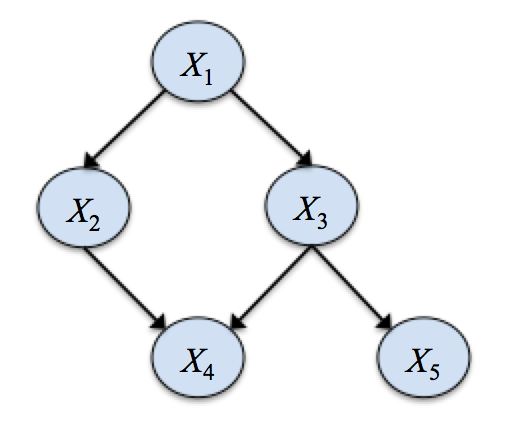
\includegraphics[scale=0.55]{./figures/ExampleBN}
\caption{\label{Figure:ExampleBN}Example of a BN model with five variables.}
\end{center}
\end{figure}

A BN is called \emph{hybrid} if some of its variables are discrete while some others are continuous. In the AMIDST modelling framework \cite{Deliverable2.1}, we specifically consider \emph{conditional linear Gaussian (CLG) BNs}\cite{Lauritzen1992,lauritzen1996graphical,LauritzenJensen2001}. In a CLG, the local probability distributions of the continuous variables are specified as CLG distributions and the discrete variables are required to only have discrete parents. From an implementation point of view, and depending on the type of the child and parent variables, i.e., discrete or continuous, it can be advantageous to distinguish between the following conditional distributions:

\vspace{-0.1in}

\begin{itemize}
\item \emph{discrete $\mid$ discrete}: the discrete child follows an independent multinomial probability distribution for each configuration of its discrete parents.

\item \emph{continuous $\mid$ discrete}: the continuous child is distributed as an independent CLG distribution for each configuration of its discrete parents. 

\item \emph{continuous $\mid$ continuous}: the continuous child follows a CLG distribution, i.e., the mean parameter of its Gaussian distribution is a linear combination of its continuous parents, while the variance is a fixed independent parameter. 

\item \emph{continuous $\mid$ (discrete, continuous)}: for each configuration of the discrete parents, the continuous child follows an independent CLG distribution depending on its continuous parents. That is, the mean parameter of the Gaussian distribution of the continuous child is expressed as a linear combination of the continuous parents for each configuration of the discrete parents.
\end{itemize}
 
%--------------------------------------------------------------------------------------------------
% 2T-DBN
%--------------------------------------------------------------------------------------------------

The second type of PGM that is considered in the AMIDST modelling framework is the dynamic Bayesian network\footnote{Remark: In this setting, dynamics refer to the time-dimension of the model, not that the model-specification changes dynamically.}(DBN)\cite{DeanKanazawa1989}. DBNs are used to model domains that evolve over time by representing explicitly the temporal dynamics of the system being modelled. DBNs can then be readily understood as an extension of standard static BNs to the temporal domain. In fact, similarly to static BNs, the problem is modelled using a set of stochastic random variables, denoted $\mathbf{X}^t$, with the main difference that variables are indexed by a discrete time index $t$, as shown in Figure \ref{Figure:ExampleDBN}.

In the AMIDST modelling framework \cite{Deliverable2.1},  we especially focus on the so-called \textit{two-time slice DBNs} (2T-DBNs). 2T-DBNs are defined by an \textit{initial model} representing the initial joint distribution of the process and a \textit{transition model} representing a standard BN repeated over time. This kind of DBN model is based on \textit{the first-order Markov} and \textit{the stationary} assumptions. The first-order Markov assumption specifies that knowing the present makes the future conditionally independent from the past, i.e., $p(\bm X^{t+1} | \bm X^{1:t})  = p(\bm X^{t+1} | \bm X^{t})$, while the stationary assumption entails that changes in the system state are time invariant or time homogeneous, i.e., $p(\bm X^{t+1}|\bm X^{t}) = p(\bm X^t|\bm X^{t-1})\ \forall t \in\{1,\ldots,T\}$. 

In a 2T-DBN, the transition distribution is represented as follows:

$$ p(\mathbf{X}^{t+1} |\mathbf{X}^t) = \prod_{X^{t+1}\in \mathbf{X}^{t+1}} p(X^{t+1}|Pa(X^{t+1}))$$ 

\noindent where $Pa(X^{t+1})$ refers to the parent set of $X^{t+1}$ in the transition model, which can be either in the same or the previous time step. Figure \ref{Figure:ExampleDBN} shows an example of a graphical structure of a 2T-DBN model. For instance, we have $Pa(X_1^{t+1}) = X_1^{t}$.

\begin{figure}[ht!]
\begin{center}
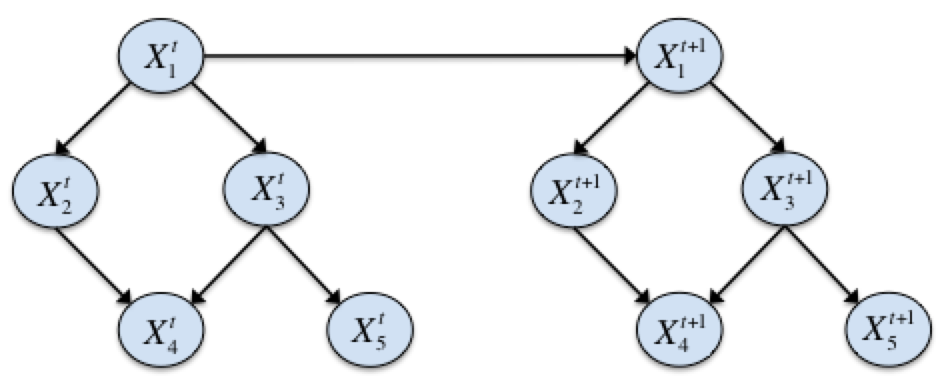
\includegraphics[scale=0.6]{./figures/ExampleDBN}
\caption{\label{Figure:ExampleDBN}An example of a BN structure corresponding to a 2T-DBN.}
\end{center}
\end{figure}

Special types of DBNs include hidden Markov models (see Deliverable 2.1\cite{Deliverable2.1}, Section 3.3.1), and Kalman or switching Kalman filter models (see Deliverable 2.1 \cite{Deliverable2.1}, Section 3.3.2).